\documentclass{beamer}
\usepackage[utf8]{inputenc}
\usepackage[T1]{fontenc}
\usepackage{lmodern}
\usepackage{ngerman}
\usepackage{bibgerm}
\usepackage{color}
\usepackage{graphicx}
\usepackage{pstricks}

\mode<presentation>  {
  \usetheme{Warsaw}
  \useoutertheme{miniframes}
  \setbeamertemplate{navigation symbols}{}
}

\newcommand{\defaultscale}{0.5}
\newcommand{\pfeil}{\item[$\Rightarrow$]}
\newcommand\ato{\rightarrow} %Morphismen

\newcommand{\sexp}{S"=Expression}
\newcommand{\sexps}{S"=Expressions}
\newcommand{\cgen}{Code"=Generierung}
\newcommand{\cpp}{C\texttt{++}}

\title[\cgen{}]{Prototyp eines universellen Frameworks für
  \sexp{}-basierte \cgen{}}
\subtitle{Diplomarbeit}
\author[Benjamin Teuber]{Benjamin Teuber\\ Erstbetreuer: Daniel Moldt}
\date{\today}
\institute{Universität Hamburg\\ 
  Fakultät für Mathematik, Informatik und Naturwissenschaften\\
  Department Informatik}

\begin{document}

\section{Einführung}
\subsection{Einführung}

\maketitle

\AtBeginSubsection{
\begin{frame}
\begin{center}
\structure{\Huge \insertsubsection}
\end{center}
\end{frame}
}

%% TODO:
%% CarXML gerade
%% R Zeichen      

\begin{frame}{Themengebiet: \cgen}
  \begin{itemize}
  \item \cgen{} immer stärker genutzt
    \begin{itemize}
    \item Model-Driven Architecture
    \item Domain-Specific Languages
    \end{itemize}
  \item Problem: Generator bauen ist aufwändig
  \item Viele Komponenten nötig 
    \begin{itemize}
    \item Parser für Quellsprache
    \item Compiler in normaler Programmiersprache
    \item Templates für Zielsprache
    \end{itemize}
  \item Ziel: Framework aus einem Guss
  \end{itemize}
\end{frame}

\begin{frame}{Inhalt}
  \begin{itemize}
  \item Vergleich bestehender Technologien
  \item Ableiten von Anforderungen
  \item Entwurf eines prototypischen Frameworks
    \begin{itemize}
    \item Architektur
    \item Komponenten
    \end{itemize}
  \end{itemize}
\end{frame}

\section{Vorhandene Technologien}
\subsection{Vorhandene Technologien}

\begin{frame}{Übersicht: Vergleich bestehender Technologien}
  \begin{itemize}
  \item Verschiedene Typisierungsgrade von Modellen
    \begin{itemize}
    \item Zeichenketten - low level
    \item Objekte - typisiert, aber unflexibel
    \item Bäumrepräsentationen wie XML oder \sexps{}
    \end{itemize}
  \item Code-Erzeugung
    \begin{itemize}
    \item Templates - verschiedene Mächtigkeiten
    \item Programmatisch - z.B. Stringmanipulationen
    \end{itemize}
  \item Kontrollfluss
    \begin{itemize}
    \item Direkter Aufruf von Templates
    \item Impliziter Aufruf über Struktur
    \end{itemize}
  \end{itemize}
\end{frame}

\begin{frame}{Untypisierte Baumrepräsentationen}
  \begin{columns}
    \begin{column}{5cm}
      \begin{itemize}
      \item Grundmodell: Bäume mit benannten Knoten und Zeichenketten als Blättern
      \item Kompromiss zwischen Flexibilität und Strukturierung
      \end{itemize}
    \end{column}
    \begin{column}{5cm}
      \begin{figure}
        \centering
        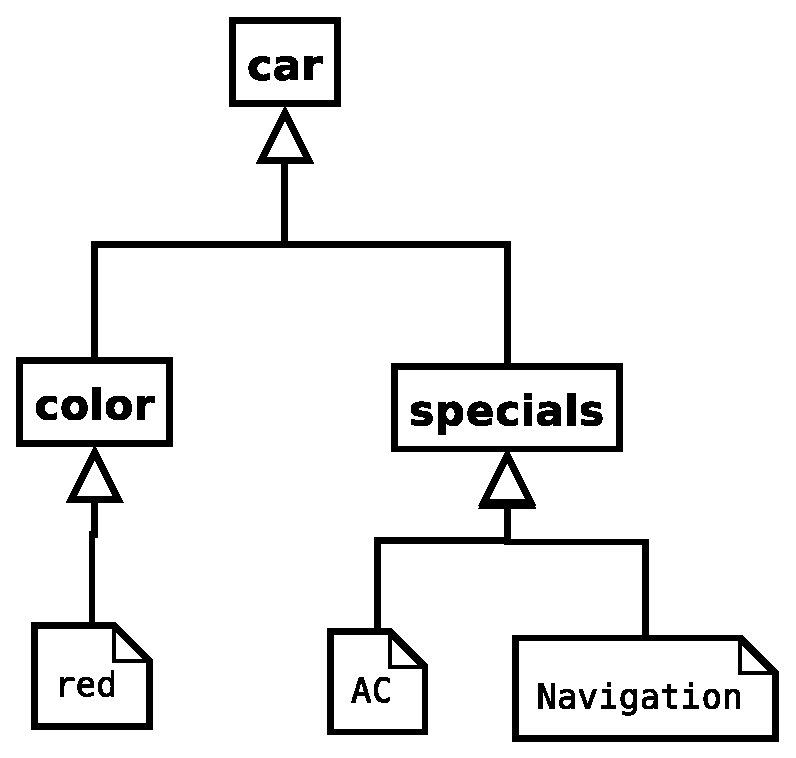
\includegraphics[scale=0.3]{images/car_sexp}
        \caption{Auto-Modell als Baum}
      \end{figure}
    \end{column}
  \end{columns}
\end{frame}

\begin{frame}{Exkursion: Lisp}
  \begin{itemize}
  \item Eine der ältesten Programmiersprachfamilien (LISP: 1958)
  \item Minimale, uniforme Syntax (S-Expressions $\simeq$ XML-Subset)
  \item Sprache selbst kann durch Makros erweitert werden \\
    ``The programmable programming language''
  \end{itemize}

  \begin{block}{Zitat}
    ``Any sufficiently complicated C or Fortran program contains an ad hoc
    informally-specified bug-ridden slow implementation of half of
    Common Lisp.''

    - Philip Greenspun 
  \end{block}
\end{frame}

\begin{frame}[fragile]{S-Expressions}
  \begin{itemize}
  \item Ein S-Expression ist entweder:
    \begin{itemize}
    \item Ein Atom, z.B. eine Zahl, ein String, eine Variable
    \item Eine Liste von S-Expressions in Notation \\ \texttt{($sexp_1$ $sexp_2$ .. $sexp_n$)}
    \end{itemize}
  \item Konvention: Knotenname an erster Stelle
  \item \textit{Strukturelle} Verarbeitung
  \item Beispiel: Funktionsdefinition in Common Lisp
  \end{itemize}
\begin{verbatim}
    (defun my-add (a b)
      (+ a b))
\end{verbatim}
\end{frame}

\begin{frame}{Kritik an XML}
  \begin{columns}
    \begin{column}{6cm}
      \begin{itemize}
      \item Verbreitetste Sprache mit Baummodell
      \item Viele zusätzliche Merkmale
        \begin{itemize}
        \item Attribute
        \item Namespaces
        \end{itemize}
      \item These: Attribute sind unnötig
        \begin{itemize}
        \item Spezielle Form von Kindern
        \item keine sinnvolle Zuordnung möglich
        \end{itemize}
      \item Problem: Keine Listen von Blättern
      \end{itemize}
    \end{column}
    \begin{column}{4cm}
      \begin{figure}
        \centering
        \includegraphics[scale=0.3]{images/car_xml}
        \caption{Auto-Modell in XML}
      \end{figure}    
    \end{column}
  \end{columns}
\end{frame}

\begin{frame}{Vorteile von \sexps{}}
  \begin{itemize}
  \item Simple Struktur - vereinfachen:
    \begin{itemize}
     \item Parsing (vgl. XML)
    \item Verarbeitung
    \item Erzeugung
    \end{itemize}
  \item Dennoch ausdrucksstark
    \pfeil Basis für Lisp-Makros
  \end{itemize}
\end{frame}

\begin{frame}[fragile]{Templates}
  \begin{itemize}
  \item Für Dokumenterzeugung genutzt
  \item ``Schablone mit Platzhaltern''
  \item Funktion: $\mathrm{input} \ato \mathrm{doc}$
  \item Unterschiede:
    \begin{itemize}
    \item Typen $\mathrm{input}$ und $\mathrm{doc}$
    \item Syntax der Metasprache
    \item Mächtigkeit
    \end{itemize}
  \end{itemize}
\end{frame}

\begin{frame}[fragile]{PHP}
  \begin{itemize}
  \item $\mathrm{Object}\ato\mathrm{String}$
  \item Zeichenketten problematisch
    \begin{itemize}
    \item Syntaxfehler
    \item Einrückung für lesbaren Code?
    \end{itemize}
  \item Komplette Programmiersprache
  \end{itemize}
\begin{verbatim}
<html>
  <head><title>Current Date</title></head>
  <body>
    <? print($current_date); ?>
  </body>
</html>
\end{verbatim}
\end{frame}

\begin{frame}[fragile]{XSL Transformation}
  \begin{itemize}
  \item $\mathrm{XML} \ato \mathrm{XML}$
  \item Mächtig, aber umständliche Syntax
    \begin{itemize}
    \pfeil Praxis: Komplexe Verarbeitung in externer
      Programmiersprache
    \end{itemize}
  \item Ermöglicht direkten Aufruf sowie Matching über XPath
  \item XPath: \verb+/book[@price>35]/title+
  \end{itemize}
\end{frame}

\begin{frame}[fragile]{XSLT (2)}

  \begin{block}{Eingabe}
\begin{verbatim}
<addresses>
  <person firstname="Heinz" name="Schulz" />
  <person firstname="Walter" name="Meier" />
</addresses>
\end{verbatim}
  \end{block}
  \begin{block}{Erwünschte Ausgabe}
\begin{verbatim}
<table>
  <tr> <td>Walter</td> <td>Meier</td> </tr>
  <tr> <td>Heinz</td> <td>Schulz</td> </tr>
</table>    
\end{verbatim}
\end{block}
\end{frame}

\begin{frame}[fragile]{XSLT (3)}
\begin{verbatim}
<xsl:template match="/addresses">
  <table>
    <xsl:for-each select="person">
      <xsl:sort select="@name" 
                order="ascending" 
                data-type="text" />
        <tr>
          <td><xsl:value-of select="@firstname" /></td>
          <td><xsl:value-of select="@name" /></td>
        <tr>
      </xsl:sort>
    </xsl:for-each>
  </table>
</xsl:template>
\end{verbatim}
\end{frame}

\begin{frame}[fragile]{Lisp-Makros}
  \begin{itemize}
  \item $\mathrm{Sexp} \ato \mathrm{Sexp}$
  \item Metasprache $=$ Zielsprache $=$ Quellsprache $=$ Lisp
  \item ``Compiler-Plugins'' in kurzer, eleganter Notation
    \begin{itemize}
    \item Ermöglichen inkrementelle Erweiterung des Lisp-Compilers
    \item ``Embedded DSLs'' - in die ursprüngliche Sprache integriert
    \end{itemize}
  \item Einschränkungen:
    \begin{itemize}
    \item Typen
    \item Kontrollfluss
    \item Kein ``SPath''
    \end{itemize}
  \end{itemize}
\end{frame}

\begin{frame}[fragile]{Lisp-Makros (2)}
  \begin{block}{Makro-Aufruf}
\begin{verbatim}
(addresses
  (person "Heinz" "Schulz")
  (person "Walter" "Meier"))
\end{verbatim}
  \end{block}
  \begin{block}{Zu erzeugender Code}
\begin{verbatim}
(table
  (tr (td "Walter") (td "Meier"))
  (tr (td "Heinz")  (td "Schulz")))
\end{verbatim}
  \end{block}
\end{frame}

\begin{frame}[fragile]{Lisp-Makros (3)}
  \begin{block}{Makro-Umsetzung in Common Lisp}
\begin{verbatim}
(defun sort-by-name (persons) ...)

(defmacro addresses (&rest persons)
  `(table ,@(sort-by-name persons)))

(defmacro person (first-name name)
  `(tr (td ,first-name) (td ,name)))
\end{verbatim}
  \end{block}
\end{frame}

\section{Anforderungen}
\subsection{Anforderungen}

\begin{frame}{MagicL}
  \begin{itemize}
  \item M: Models
  \item A: Architecture
  \item G: Generation
  \item I: Interface
  \item C: Control Flow
  \item L: Lisp
  \end{itemize}
\end{frame}

\begin{frame}{Anforderungen}
  \begin{itemize}
  \item Lisp
    \begin{itemize}
    \item Makro-Ansatz
    \end{itemize}
  \item Modelle
    \begin{itemize}
    \item \sexps{}
    \item Objekte
    \item Strings
    \end{itemize}
  \item Generierung von Quelltext
    \begin{itemize}
    \item Nicht auf Zeichenketten-Ebene
    \item Modell für Code
    \item automatische Formatierung
    \end{itemize}
  \end{itemize}
\end{frame}

\begin{frame}{Anforderungen (2)}
  \begin{itemize}
  \item Architektur
    \begin{itemize}
    \item theoretische Fundierung
    \item visualisierbar (vgl. Petri-Netze)
    \item flexible Verarbeitungsprozesse
    \end{itemize} 
  \item Compiler-Schnittstelle
    \begin{itemize}
    \item universell - Parser, Makros
    \item automatische Auswahl über Typ
    \end{itemize}
  \item Kontrollfluss für Makros
    \begin{itemize}
    \item direkter Aufruf
    \item impliziter Aufruf durch Matching
      \begin{itemize}
      \item XPath?
      \item EBNF?
      \end{itemize}
    \end{itemize}    
  \end{itemize}
\end{frame}

\section{Architektur}
\subsection{Architektur}

\begin{frame}[fragile]{Die Sprache Haskell}
  \begin{itemize}
  \item Funktional (pur)
  \item statische Typinferenz
  \item Typklassen entsprechen Java-Interfaces
  \item Seiteneffekte dank Monaden/Arrows integrierbar
  \end{itemize}
\begin{verbatim}
getName :: IO String
getName = return "Harald"

main :: IO ()
main = do name <- getName
          putStrLn name
\end{verbatim}
\end{frame}

\begin{frame}{Kategorientheorie}
  \begin{itemize}
  \item Sehr abstrakter Bereich der Mathematik
    \begin{itemize}    
    \item Praktisch alle mathematischen Strukturen sind Kategorien
    \item Motivation: ``Rechnen mit Funktionstypen''
    \end{itemize}
  \item Morphismen zwischen Objekten: $f: \mathrm{A} \ato \mathrm{B}$
    \begin{itemize}
    \item Interpretation frei
    \item Komposition: $g \circ f$ analog Funktionen
    \item Identität: $\mathrm{id}_{A}$
    \item Produkte ($f \times g$) und Coprodukte ($f + g$)
    \end{itemize}
  \item Funktoren: Abbildungen zwischen Kategorien
  \item Weiteres: Natürliche Transformationen, Monaden etc.
  \end{itemize}
\end{frame}

\begin{frame}{Kategorien in Haskell}
  \begin{itemize}
  \item Objekte: Haskell-Datentypen 
  \item Arrows: Verarbeitungsprozesse
    \begin{itemize}
    \item pure Funktionen (Kategorie $\mathbf{Hask}$)
    \item Funktionen mit Side-Effects ($\mathbf{IOArrow}$)
    \end{itemize}
  \item eigene Arrow-Formalismen möglich
    \begin{itemize}
    \item müssen Komposition etc. implementieren
    \item Funktor von $\mathbf{Hask}$ erforderlich
    \end{itemize}
  \end{itemize}
\end{frame}

\begin{frame}{Funktoren in dieser Arbeit}
  \begin{itemize}
  \item Gleicher Arrow in verschiedenen Kategorien
    \begin{itemize}
    \item Unterschiedliche Typsignatur möglich
      \pfeil ``Verstecken'' von Teilen der Signatur
    \end{itemize}
  \item ``Domain Specific Categories''
  \item Beispiel 1: Möglichkeit zum Scheitern ($\mathbf{C}_F$)
    \begin{itemize}
    \item in $\mathbf{C}_F: \mathrm{A} \ato \mathrm{B}$
    \item in $\mathbf{C}: \mathrm{A} \ato \mathrm{B} + \mathrm{String}$
    \end{itemize}
  \item Beispiel 2: Zustände ($\mathbf{C}_S$)
    \begin{itemize}
    \item in $\mathbf{C}_S: \mathrm{A} \ato \mathrm{B}$
    \item in $\mathbf{C}: \mathrm{A} \times \mathrm{state} \ato \mathrm{B} \times \mathrm{state}$
    \end{itemize}
  \end{itemize}
\end{frame}

\begin{frame}{Überblick Architektur}
  \begin{itemize}
  \item Komplett Arrow-basiert
    \begin{itemize}
      \pfeil Generische Schnittstelle für alle Arten von Compilern
    \end{itemize}
  \item Compiler: $\mathrm{a} \ato \mathrm{b}$
  \item Parser: $\mathrm{[token]} \ato \mathrm{b}$ 
  \item Makros: $\mathrm{[Sexp]} \ato \mathrm{b}$ 
  \item Lisp-Makros: $\mathrm{[Sexp]} \ato \mathrm{[Sexp]}$
  \end{itemize}
\end{frame}

\begin{frame}{Parser als Arrows}
  \begin{itemize}
  \item Eigenschaften von Parsern:
    \begin{itemize}
    \item Fehlschlagen / Alternativen ($\Rightarrow \mathbf{C}_F$)
    \item Zustand: Position im Eingabestream ($\Rightarrow \mathbf{C}_S$)
    \end{itemize}
  \item Kombination: $\mathbf{C}_P = \mathbf{C}_{FFS}$
    \begin{itemize}
    \item ``innerer Fail'' möglich
      \pfeil bessere Fehlermeldungen
    \end{itemize}
  \end{itemize}
\end{frame}

\begin{frame}{Parser als Arrows (2)}
  \begin{itemize}
  \item Signaturen eines Parsers
    \begin{itemize}
    \item Parser-Kategorie: $\emptyset \ato \mathrm{A}$
    \item ``Wirklichkeit'': $[\mathrm{token}] \ato (\mathrm{A} \times
      [\mathrm{token}] + \mathrm{String}) + \mathrm{String}$
    \item nach Umwandlung in Compiler: $[\mathrm{token}] \ato \mathrm{A}$
    \end{itemize}  
  \item Token-Typ Variabel: $\mathrm{Char}$ und $\mathrm{Sexp}$
    verwendet
  \end{itemize}
\end{frame}

\begin{frame}[fragile]{Parser-Bibliothek}
  \begin{itemize}
  \item Kombinatoren: \verb+empty, eq, member, many, optional etc.+
  \item Aufruf innerer Parser: \verb+applyParser+
    \pfeil Makros:
\begin{verbatim}
  macro "addresses" (many (macro "person" 
                                 compSymbol 
                                 compSymbol))
\end{verbatim}
  \end{itemize}
\end{frame}

\section{Komponenten}
\subsection{Komponenten}

\begin{frame}{Komponenten von MagicL}
  \begin{itemize}
  \item Modelle
    \begin{itemize}
    \item Sexp
    \item Code
    \end{itemize}
  \item Eigene DSLs
    \begin{itemize}
    \item \sexp{}-Haskell
    \item \sexp{}-Compiler
    \end{itemize}
  \item Außerdem
    \begin{itemize}
    \item minimales Test-Framework
    \item Build-Tool
    \end{itemize}
  \end{itemize}
\end{frame}

\begin{frame}[fragile]{Parser: $\mathrm{String} \ato \mathrm{Sexp}$}
\begin{verbatim}
data Sexp = Symbol String
          | Node   [Sexp]

whitespace = skip (many (member " \t\n"))

parseSymbol = many1 (notMember " \t\n()") >>>
              symbol

parseNode = skip (eq '(') >>> 
            (many parseSexp >>> node) >>> 
            skip (eq')')

parseSexp = whitespace >>> 
            (parseSymbol <+> parseNode) >>> 
            whitespace
\end{verbatim}
\end{frame}

\begin{frame}[fragile]{Quellcode-Modell}
  \begin{itemize}
  \item Ansatz von Philip Wadler
  \item Beschreibung durch Haskell-Funktionen
    \begin{itemize}
    \item Elementar: \verb+text, newline, indent, append, group+
    \item Abgeleitet: \verb+lines, paragraphs, parens etc.+
    \end{itemize}
  \item Beispiel: Pretty-Printer für \sexps{}
  \end{itemize}
\begin{verbatim}
layoutSexp :: Sexp -> Code
layoutSexp (Symbol sym) = text sym
layoutSexp (Node children) = 
    format (map layoutSexp children)
  where format = parens . group . indent2 . lines
\end{verbatim}
\end{frame}

\begin{frame}[fragile]{Sexp-Haskell}
  \begin{itemize}
  \item Ziel: \sexp{}-basierte Erzeugung von Haskell-Code
  \item Ansatz: Haskell-Variante in \sexp{}-Syntax
  \end{itemize}
  \begin{columns}
    \begin{column}{5cm}
      \begin{block}{Sexp-Haskell}
\begin{verbatim}
(= (sumOfSquares x y)
   (+ x2 y2)
 (where                   
  (= x2 (* x x))
  (= y2 (* y y))))
\end{verbatim}
      \end{block}
    \end{column}
    \begin{column}{6cm}
      \begin{block}{Haskell}
\begin{verbatim}
sumOfSquares x y = (x2 + y2)
  where
    x2 = (x * x)         
    y2 = (y * y)
\end{verbatim}
      \end{block}
    \end{column}
  \end{columns}
\end{frame}

\begin{frame}[fragile]{Implementation von Sexp-Haskell}
  \begin{itemize}
  \item Zeigt Einbindung typisierter Modelle
  \item Drei Komponenten
    \begin{itemize}
    \item Haskell-Modell
    \item Parser $\mathrm{Sexp} \ato \mathrm{Haskell}$
    \item Funktionaler Compiler $\mathrm{Haskell} \ato \mathrm{Code}$
    \end{itemize}
  \item Nutzt automatisches Finden von Compilern
  \pfeil Formulierung etwas umständlich
  \end{itemize}
\end{frame}

\begin{frame}[fragile]{Haskell-Modell}
\begin{verbatim}
...

data Pattern = ListPattern [Pattern]
             | TuplePattern [Pattern]
             | ConsPattern [Pattern]
             | StringPattern String
             | CallPattern Call                          

...
\end{verbatim}
\end{frame}

\begin{frame}[fragile]{$\mathrm{Sexp} \ato \mathrm{Haskell}$}
\begin{verbatim}
...

instance Compilable (SexpParser Pattern) [Sexp] Pattern 
 where
  comp =
    (liftA1 ListPattern (macro "List" comp)   <+>
     liftA1 TuplePattern (macro "Tuple" comp) <+>
     liftA1 ConsPattern (macro "Cons" comp)    <+>
     liftA1 StringPattern (macro "Str" (many comp >>^ 
                                        unwords)) <+>
     liftA1 CallPattern comp)

...
\end{verbatim}
\end{frame}

\begin{frame}[fragile]{$\mathrm{Haskell} \ato \mathrm{Code}$}
\begin{verbatim}
...

instance Compilable (Pattern -> Code) Pattern Code where
  comp (ListPattern pats)  = list $ map comp pats
  comp (TuplePattern pats) = tuple $ map comp pats
  comp (ConsPattern pats)  = parenFoldOp ":" (map comp
                                                  pats)
  comp (StringPattern str) = string str
  comp (CallPattern call)  = comp call
...

\end{verbatim}
\end{frame}

\begin{frame}[fragile]{Sexp-Compiler}
  \begin{itemize}
  \item DSL für untypisierte \sexp{}-Verarbeitung ähnlich Lisp
    \begin{itemize}
    \item Quasiquote-Operator für \sexp{}-Templates
    \item Makro-Typ: $\mathrm{[Sexp]} \ato \mathrm{[Sexp]}$
    \item Lisp-Kontrollfluss: Auto-Makros
    \end{itemize}
  \item Metarekursiv implementiert
  \end{itemize}
  \begin{block}{Beispiel: Mehrere Rückgaben}
\begin{verbatim}
(autoMac compDefArith defArithFuns
  (' (= (add x y) (+ x y))
     (= (sub x y) (- x y))))
\end{verbatim}
  \end{block}
\end{frame}

\section{Schluss}
\subsection{Schluss}

\begin{frame}{Zusammenfassung}
  \begin{itemize}
  \item Prototyp eines universellen Compiler-Frameworks
  \item Sauber fundiert: Haskell, Kategorientheorie
  \item Lisp-inspiriert: \sexps{}, Makros
  \item Allgemeiner
    \begin{itemize}
    \item Modelltypen
    \item Verarbeitungsprozesse
    \item Kontrollfluss
    \end{itemize}
  \end{itemize}
\end{frame}

\begin{frame}{Ausblick}
  \begin{itemize}
  \item Compiler-Definitionen sind etwas redundant
    \pfeil Plan: DSL für Modelldefinitionen
  \item Code-Modell in \sexps{}
  \item Unterstützung verschiedener Zielsprachen
  \item \sexp{}-basierte Softwareentwicklung
    \begin{itemize}
    \item Datenbank
    \item Strukturelle IDE
    \item Anpassbare Visualisierung
    \pfeil Model-View-Trennung von Code
    \end{itemize}
  \end{itemize}
\end{frame}

\begin{frame}
  \begin{center}
    \Huge Vielen Dank für die Aufmerksamkeit!
  \end{center}
\end{frame}

\end{document}
